\label{ch:DNN}
\section{Why Neural Networks?}

The methods discussed up to now are called \textit{tabular methods}. This means that we are actually saving values of the value function is in a table, which is a very easy way. However, tabular methods are usable only in very low dimensionality problems, otherwise, the amount of memory required to store all the data would be extremely large. Additionally, when trying to look up for a value of a particular state, it will require an entire sweep of the table which is computationally expensive. Moreover, if the state space is continuous, a tabular format is impossible. To overcome this problem, \textit{function approximators} are used to store value functions.
\\
\indent Many function approximation algorithms have been developed over the years, but one of the most recent breakthroughs in Machine Learning was the development of \textit{Deep Neural Networks (DNNs)}. These methods have given a surge in the field of Reinforcement Learning algorithms, and have paved the way for successfully carrying out tasks that were once considered impossible, such as the AlphaGo project\cite{silver2017mastering}.

\section{Building Units}

	Artificial neural networks are inspired and loosely modeled after how the human brain works. The human brain is a complex web of interconnected neurons, its building units, which is capable of extracting critical information from the inputs and producing a corresponding output (signal). In a similar way, a Deep Neural Network consists of a set of interconnected neurons, arranged in layers, where each neuron takes some real value input and gives a real valued output. 

\begin{figure}
	\centering
	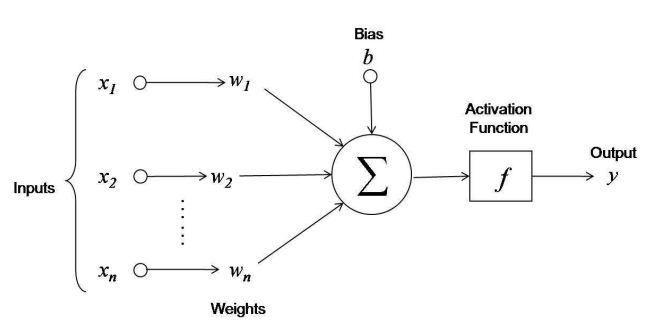
\includegraphics[width=10cm]{images/NeuronDiagram}
	\caption{An artificial neuron}
	\label{fig:neuron}
	
% NOTE: WE CAN INSERT JUST A LINK OF CITATION TO THE IMAGE! AS IN THE LEO THESIS

\end{figure}

\subsection{Artificial Neuron}
Figure \ref{fig:neuron}\footnote{\href{https://medium.com/@jayeshbahire/the-artificial-neural-networks-handbook-part-4-d2087d1f583e}{Source: medium.com}} shows an artificial neuron. The neuron takes as input a vector of inputs $x = [x_1, x_2, ..., x_n]$ and calculates a weighted sum of the inputs, with the neuron \textit{weights} denoted by the vector $w_i = [w_{i,1}, w_{i,n}, ..., w_{i,n}]$, which is actually the $i_{th}$ row of a weight matrix. The weighted sum is then added to a \text{bias} term, $b$, and then is passed through an \textit{activation function}, $f$, which produces the output of the neuron. Our  complete equation for a single neuron can be written as:


\begin{equation}
	\label{eq:neuron}
	y_i = f(\sum_{j} x_j w_{i,j} + b_i)
\end{equation}

where $j$ is the number of inputs to the neuron, and $i$ represents the $i_{th}$ layer of neurons of the DNN.
\\
\indent What we can see here is that a single neuron carries indeed a non-linear function, and the interconnecting of many neurons gives the DNN a great complexity, but it also enables it to be a very powerful tool. Indeed, even if the single neuron is modeled after the biological one, since biological neurons have thousands of connections with neighboring ones and also have the ability of destroying and creating connections, they are still far more efficient than even state-of-the-art Deep Neural Networks as of writing time.

\subsection{Activation Functions}
\label{subsec:ActivationFunctions}
The activation function introduces non-linearity to the output of a neuron: this is extremely important for the network in order to learn non-linear representations from the training data. In literature, a number of activation functions have been introduced, like \textit{sigmoid}, \textit{hyperbolic tangent}, and \textit{rectified linear unit}. These commonly used activation functions are explained below:

\begin{itemize}
	\item Sigmoid: 
	\begin{equation}
		f(x) = \dfrac{1}{1 + e^{-x}}	\end{equation}
\end{itemize} 

\begin{itemize}
	\item Hyperbolic Tangent: 
	\begin{equation}
	f(x) = \dfrac{e^x - e^{-x}}{e^x + e^{-x}}	\end{equation}
\end{itemize} 

\begin{itemize}
	\item Rectified Linear Unit (ReLu)\cite{nair2010rectified}: 
	\begin{equation}
	f(x) = \max(0,x)
	\label{eq:ReLu}	
	\end{equation}
\end{itemize} 

 Since ReLu does not suffer from saturation as compared to the other two functions discussed above, it is the one providing the best performance over a wide variety of tasks.

\section{Feed Forward Networks}
\label{sec:feedforward}
The most common architecture used in DNN is the \textit{Feed-Forward} neural networks. Figure \ref{fig:feedforward}\footnote{\href{http://cse22-iiith.vlabs.ac.in/exp4/index.html}{Source: vlabs.ac.in}} shows an example of this architecture.

\begin{figure}[h]
	\centering
	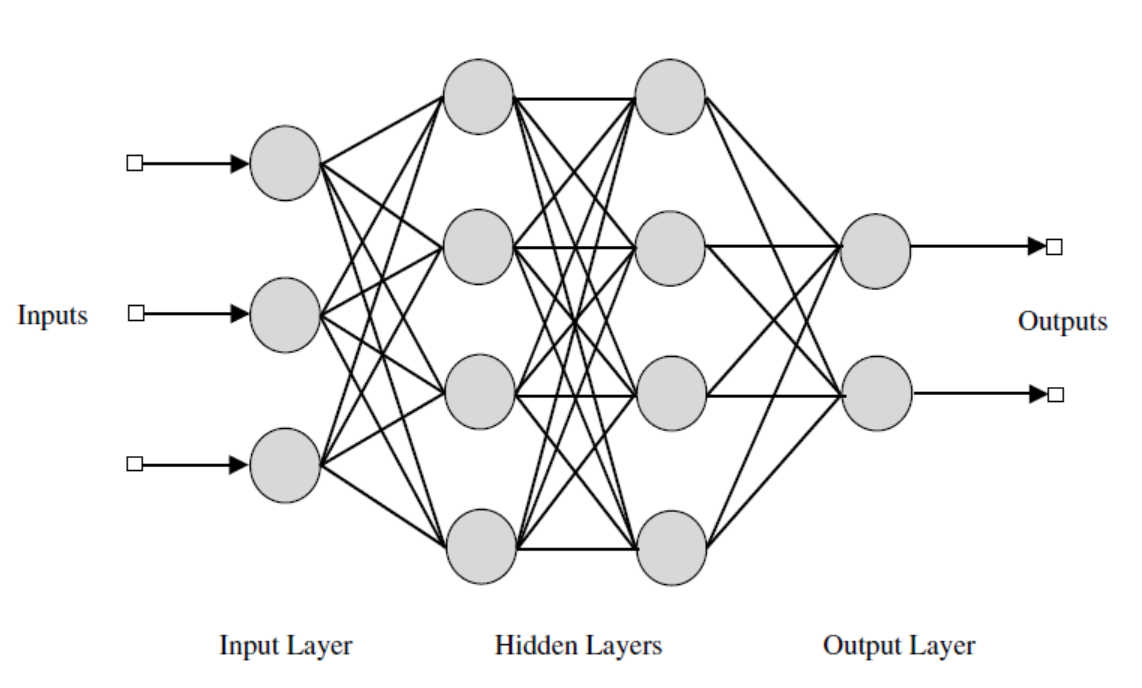
\includegraphics[width=10cm]{images/FeedForward}
	\caption{A Feed Forward neural network with two hidden layers}
	\label{fig:feedforward}
	% NOTE: WE CAN INSERT JUST A LINK OF CITATION TO THE IMAGE! AS IN THE LEO THESIS
	
\end{figure}

In this framework, neurons are arranged in three kinds of layers:

\begin{itemize}
	\item One \textit {input layer}: where the flow of information begins, this is the layer taking the raw input: therefore, the number of input neurons will be equal to the number of input features.
	\item One or more \textit{hidden layers}: these may have a variable number of neurons, and they serve as an intermediate stage between inputs and outputs making the neural network able to predict more complex outputs. \textit{Deep} NNs are called like this because of the hidden layers.
	\item One \textit{output layer}: where the flow of information ends, this is the layer predicting the outputs: neuron number will be equal to the number of output features.
\end{itemize}

Each single neuron in the different layers performs the computation shown in Equation \ref{eq:neuron}.

\subsection{Training the Network}
\label{subsec:traininnet}

The weights of the neural network are trained with a technique known as \textit{backpropagation}. The idea of this approach is the initialization of the network with random weights and then the calculation the output for a given input. Initially, since the network has not been trained yet, it will produce a random output. The error between the generated output and the actual output is used to update the weights using a gradient descent algorithm: the error function will gradually be minimized, so will the error between the generated and the actual output. This way, we will have successfully approximated the function we have trained the network on. Since the weights are first updated on the output layer and then propagated back into the network, the technique is known as backpropagation.
\\
\indent In recent years, a number of new training techniques have been introduced. One of the most popular choices has been the \textit{stochastic gradient descent}, but new improved versions have been successfully developed, like \textit{ADAM (A Method for Stochastic Optimization)}\cite{kingma2014adam}. These methods have advantages over using the traditional gradient descent because they can vary learning rates based on the distribution of training data. This is very convenient since they reduce the need for careful choice of the learning rate, which in turn allows a faster convergence of the algorithm.

\subsection{Underfitting and Overfitting}
\label{sec:overfitting}

Two of the most common problems which can be encountered in neural networks are underfitting and overfitting, shown in Figure \ref{fig:fitting}\footnote{Source: \href{https://medium.com/greyatom/what-is-underfitting-and-overfitting-in-machine-learning-and-how-to-deal-with-it-6803a989c76}{medium.com}}.

\begin{figure}[h!]
	\centering
	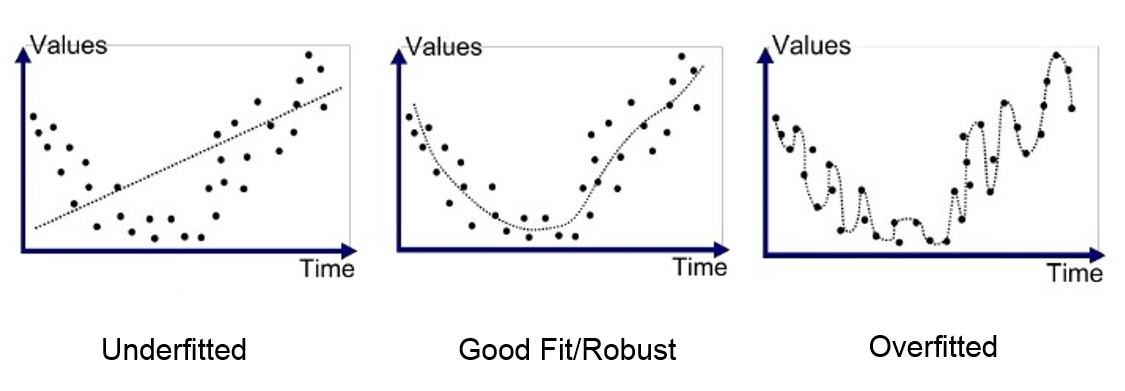
\includegraphics[width=10cm]{images/UnderOverFitting.png}
	\caption{Examples of underfitted, good fit and overfitted networks}
	%https://cdn-images-1.medium.com/max/1200/1*_7OPgojau8hkiPUiHoGK_w.png
	\label{fig:fitting}
\end{figure}

\textit{Underfitting} is a situation in which our network cannot approximate the function in a good way; in other words, the model is too simple for describing a complex data distribution. One way of reducing this problem is to increase the degree of the polynomial describing our function, so that it will approximate the function shape in a better way.
\\
\indent \textit{Overfitting} is, in a sense, the opposite of underfitting: it is a situation in which the network's model approximates the function in a "too good to be true" way. In this case the problem is that the model learned cannot generalize to new data, since it was trained too well on the training data. To overcome this problem, there are a number of solutions, such as \textit{Regularization} and \textit{Dropout}.

\section{Convolutional Neural Networks}

Convolutional Neural Networks (CNN) are an evolution of Feed Forward NNs which are able to deal with inputs of very high dimensionality. One of the most important uses for CNNs is image recognition, because indeed images are high dimensionality tensors. For example, a very simple square Grayscale image of 28 pixels is a 28x28x1 tensor, and if we had to flatten it for feeding to a classical feed forward network, the number of neurons required would be simply too high for a network to be efficient. Therefore, CNNs were developed for dealing with such problems.

\subsection{CNN Architecture}
Figure \ref{fig:CNN}\footnote{Source: \href{https://towardsdatascience.com/a-comprehensive-guide-to-convolutional-neural-networks-the-eli5-way-3bd2b1164a53}{Source: towardsdatascience.com}} shows a simple CNN for recognizing hand-written digits, which is used frequently for a first approach in learning neural networks. Among with some building blocks we have already seen, these are the main architecture component for a Convolutional Neural Network:

\begin{figure}[h]
	\centering
	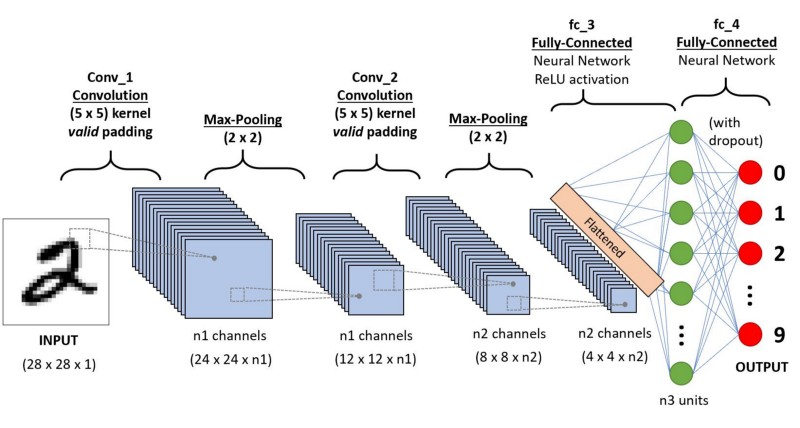
\includegraphics[width=11cm]{images/CNN.jpeg}
	%https://towardsdatascience.com/a-comprehensive-guide-to-convolutional-neural-networks-the-eli5-way-3bd2b1164a53
	\caption{A CNN for recognizing hand-written digits}
	\label{fig:CNN}
\end{figure}

%ASK FOR HOW TO DEAL WITH THIS PART

\begin{itemize}
	\item \textit{Convolutional layers}: Convolutional layers are the core building blocks of CNNs. They build up on the idea of fully connected layers we have seen before, with the main difference being they are much more computationally efficient, especially for image processing. The layers parameters consist of a set of learnable \textit{filters} (also called \textit{kernels}): they are \textit{convolved} across the width and height of the input volume (the filter is forward passed above each of the image pixels), computing the dot product between the parameters of the filter and the input, producing a 2-dimensional activation map of that filter. 
	\\
	\indent The network works by learning filters activating when they detect specific types of features at some spatial position for the input.
	\item \textit{Pooling layers}: These are another type of fundamental building blocks in CNN. A pooling layer is a form of non-linear down-sampling: it is able to reduce the memory usage, the amount of computation in the network, and it is also useful for controlling overfitting. It is common to insert a pooling layer among two successive convolutional layers. 
	\\
	\indent A common type of these layers is the \textit{max pooling}: it basically splits an image into a series of squares, each made of a number of pixels, and then downsamples it by taking the maximum of each group of pixels. For instance, if we have a 24x24 layer, a possible max pooling layer would divide it into 2x2 squares, take the maximum among them, and then producing a final layer of 12x12 made up of the maximums. This greatly reduces the computational requirements of the architecture.
	%\item \textit{Flattening}:
	
	\item \textit{Activation layers}: These layers apply non-linearities in the neural network. As we have already seen in Section \ref{subsec:ActivationFunctions} , a non-saturating activation function which has proven to be very efficient is the ReLu\cite{nair2010rectified} (Equation \ref{eq:ReLu}).
	 
	\item  \textit{Fully connected layers}: These layers carry out the high-level reasoning in the neural network, after several convolutional and pooling layers. Neurons in a fully connected layer have connections to all activations in the previous layer, as seen in the Feed Forward networks (Section \ref{sec:feedforward}). The fully connected layer is then connected to the output layer. In this section is possible to apply well known feed forward NNs techniques, for instance in preventing overfitting such as the \textit{dropout}\cite{srivastava2014dropout} technique.
\end{itemize}

\subsection{Applications}

Convolutional Neural Networks have been used for several years in many fields. They have proven to be a great tool in \textit{image recognition} systems, in which they find the most important application to date. 
\\
\indent Another frequently used implementation for CNNs is \textit{video classification}, in which the networks were found to be very efficient. The techniques basically implement image recognition to video inputs which are indeed a stream of frames one after another. 
\\
\indent \textit{Signal elaboration} is a research field in which CNNs are being used more and more. The vast complexity of the signal domain is an ideal case to be handled by this NN architecture, given its ability to decrease the need of overly-powerful computers.
\\
\indent For the purposes outlined in this thesis, an important use for Convolutional Neural Networks is the \textit{Reinforcement Learning} field. Aside of the early CNNs breakthroughs in the checkers game and the more recent development with AlphaGo\footnote{Source: \href{https://deepmind.com/research/alphago/}{deepmind.com}}, a direct implementation of CNNs along with Q-Learning are the Deep Q-Networks (DQNs, Section \ref{sec:DQN}), which have proven reliable in learning directly from high-dimensional sensory inputs.